% 设置页码计数器为 1 (也就是当前页面为第一页)
\setcounter{page}{1}

% ==================================================
% @brief    问题重述
% --------------------------------------------------

\mcmSection{问题重述}

\mcmSubsection{问题背景}

多波束测线技术是用来测量水体深度的技术。利用该技术,可以绘制出海床的地形图。规划航行路线,可以绘制出一定区间内的区域。但是海床的地形差异变化巨大,深浅不一会导致测绘系统的覆盖区域发生改变。如果测线过于密集,那么就会导致数据量过大,地形图绘制效率低下;如果过于稀疏,那么数据量过少,海床的某些区域没有探测到,地形图的绘制就会存在缺损。为了解决该问题,需要建立相关数学模型,规划测线路径,提高效率的同时,保证地形图绘制的准确性。

\mcmSubsection{具体问题重述}

\textbf{问题1:}已知相邻两个测线的截面图,如下图。其中,相邻两条测线的间距$d$、换能器开角$\theta$、坡度$\alpha$和其中一个部分的海水深度$D_0$均已知。需要利用平面几何的方法,对于不同的测线距中心点处的距离,分别求解出\textbf{海水深度}$D$、\textbf{覆盖宽度}$W$和相邻两条测线测得结果的\textbf{重叠率}$\eta$。

\begin{figure}[h]   
    \centering
    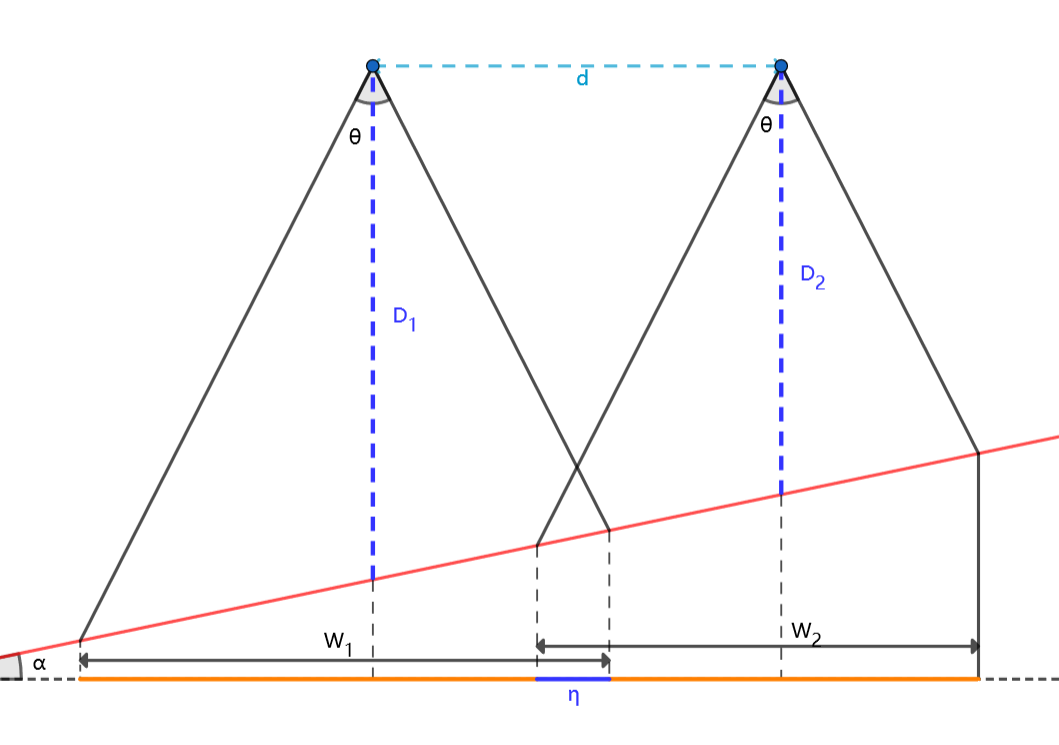
\includegraphics[scale=0.3]{res/img/问题一重述图.png}
    \caption{问题一重述图}
    \label{fig:问题一重述图}
\end{figure}

\textbf{问题2:}如下图为一个三维空间。其中,相邻两条测线的间距$d$、换能器开角$\theta$、坡度$\alpha$和其中一个部分的海水深度$D_0$均已知。需根据题意,抽象出二维平面,即将经过船且垂直于测线的平面截面置于二维平面上。再利用与问题1类似的平面几何解法,进而对于不同的测线距中心点处的距离及测线的方向角$\beta$,分别求解出\textbf{覆盖宽度}$W$。

% \begin{figure}[h]   
%     \centering
%     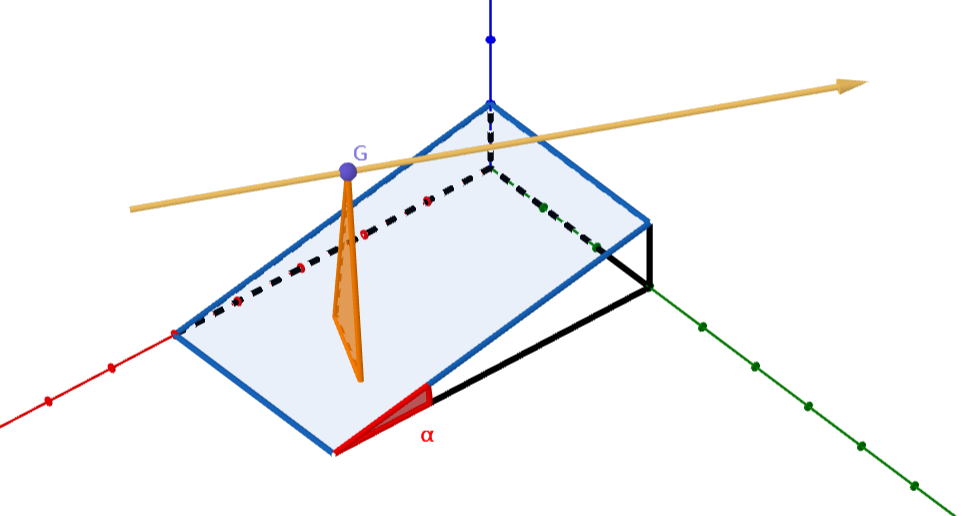
\includegraphics[scale=0.3]{res/img/问题二重述图.png}
%     \caption{\href{https://www.geogebra.org/m/pwzyn5ba}{\textcolor{blue}{问题二立体图}}}
%     \label{fig:问题二立体图}
% \end{figure}

% \begin{figure}[h]   
%     \centering
%     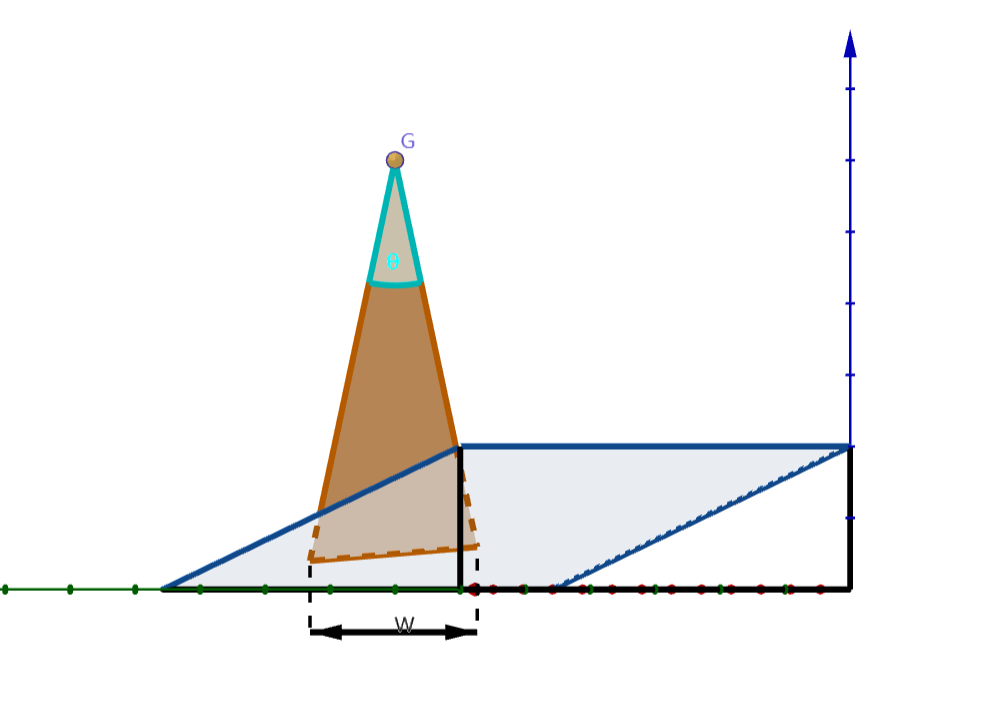
\includegraphics[scale=0.3]{res/img/问题二重述图_截面图.png}
%     \caption{\href{https://www.geogebra.org/m/g2rwmqvx}{\textcolor{blue}{问题二截面正视图}}}
%     \label{fig:问题二截面正视图}
% \end{figure}

\begin{figure}[htbp]
    \centering
    \begin{subfigure}[b]{0.45\textwidth}
      \centering
      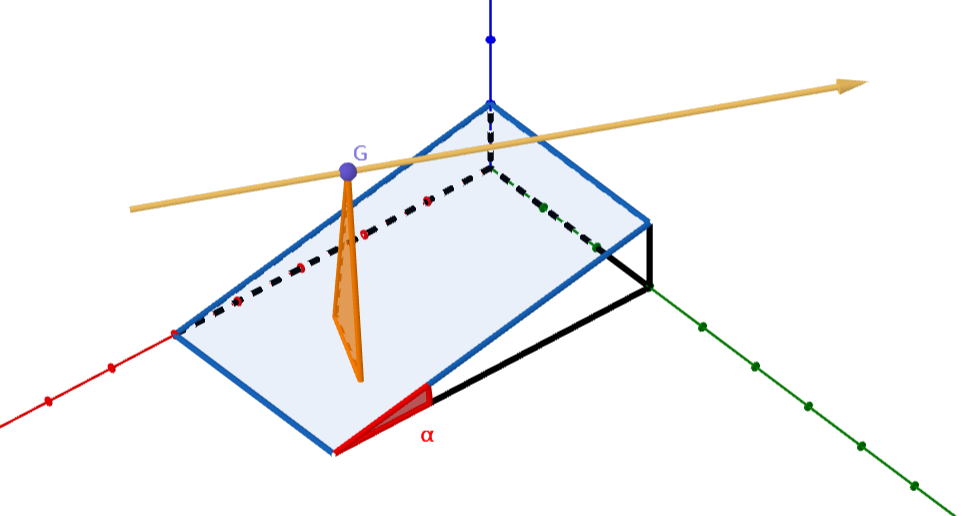
\includegraphics[scale=0.18]{res/img/问题二重述图.png}
      \caption{\href{https://www.geogebra.org/m/pwzyn5ba}{\textcolor{blue}{问题二立体图}}}
      \label{fig:问题二立体图}
    \end{subfigure}
    \hfill
    \begin{subfigure}[b]{0.45\textwidth}
      \centering
      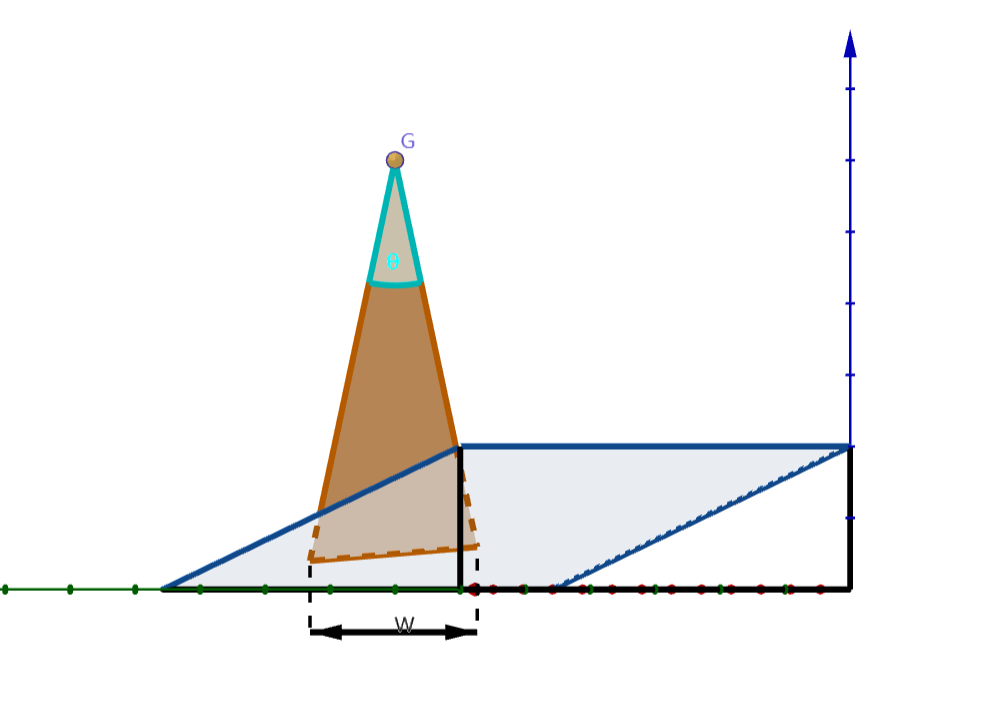
\includegraphics[scale=0.18]{res/img/问题二重述图_截面图.png}
      \caption{\href{https://www.geogebra.org/m/g2rwmqvx}{\textcolor{blue}{问题二截面正视图}}}
      \label{fig:问题二截面正视图}
    \end{subfigure}
    \caption{问题二重述图}
    \label{fig:问题二重述图}
\end{figure}

\textbf{问题3:}该问题依旧是在三维空间下的,依旧是换能器开角$\theta$、坡度$\alpha$和其中一个部分的海水深度$D_0$均已知。但是和问题二不同的是,这次需要决定:在测线的覆盖范围为整个规定海域,且重叠率$\eta \in [10\%, 20\%]$的前提下,求出测量长度最短的方案的\textbf{测线的方向角}$\beta$与相邻两条\textbf{测线的间距}$d$(允许任意两对两条相邻的测线不等距)。

\textbf{问题4:}该问题在问题3的基础上,将\textbf{坡面}更换成\textbf{不规则地形}。由于很难将整个海域一点不落地覆盖,该题要求扫描条带\textbf{尽可能}地覆盖整个海域、重叠率$\eta$\textbf{尽可能}控制在$20\%$以下和测量路线\textbf{尽可能}短。给定离散的二维平面上的点对应的海水深度数据,要求给定一个方案的\textbf{测线的方向角}$\beta$与相邻两条\textbf{测线的间距}$d$以满足要求(允许任意两对两条相邻的测线不等距)。

% ==================================================
% @brief    问题分析
% ==================================================

\mcmSection{问题分析}

\mcmSubsection{通过三角函数关系求出覆盖宽度}


% ==================================================
% @brief    模型假设
% ==================================================

\mcmSection{模型假设}

\begin{enumerate}
    \item 假设一
    \item 假设二
    \item 假设三
\end{enumerate}

% ==================================================
% @brief    模型假设
% ==================================================

\mcmSection{符号说明及名称定义}

\mcmSubsection{名称定义}

\begin{enumerate}
    \item \textbf{测垂面}是指与测线方向垂直的平面(如图\ref{fig:符号说明}中平面$GIH$);
    \item \textbf{测坡线}是指测线的测垂面与海底坡面的交线(如图\ref{fig:符号说明}中线段$IH$);
    \item \textbf{测坡角}是指测坡线与水平面的夹角(如图\ref{fig:符号说明}中线段$IH$与水平面的夹角);
    \item \textbf{海底坡面的倾斜角}是指海底坡面与水平面的夹角(如图\ref{fig:符号说明}中$\alpha$角)。\newline

    \begin{figure}[h]
        \centering
        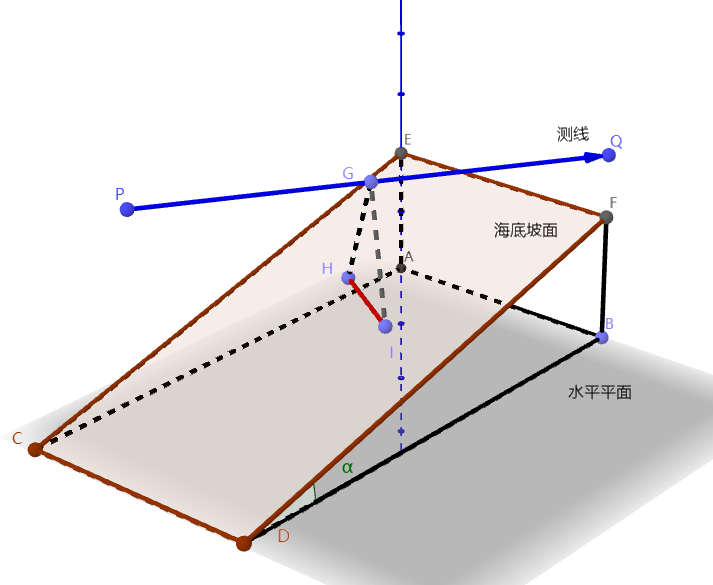
\includegraphics[scale=0.4]{res/img/符号说明.png}
        \caption{\href{https://www.geogebra.org/m/ftk9cu9v}{\textcolor{blue}{符号说明}}}
        \label{fig:符号说明}
    \end{figure}
    
\end{enumerate}


\mcmSubsection{符号说明}

\begin{table}[h]
    % 表格居中
    \centering

    % 调整行距
    \renewcommand\arraystretch{1.5}
    
    % 放缩表格
    \scalebox{1.2}{

        \begin{tabular}{cc}
        \hline
        \textbf{\fontsize{13}{1.5}{符号}}            & \textbf{\fontsize{13}{1.5}{意义}}                       \\ \hline

        $\alpha$       & 海底坡面的倾斜角     \\
        $\beta$        & 测线的方向角 \\
        $\gamma$       & 测坡角 \\ 
        $\eta$  & 覆盖率 \\ 
        $\varepsilon$  & 平坦率 \\ \hline
        \end{tabular}
    
    }
\end{table}
